\documentclass[a4paper]{article}

\usepackage[english]{babel}
\usepackage[utf8]{inputenc}
\usepackage{fullpage}
\usepackage{amsmath}
\usepackage{graphicx}
\usepackage[colorinlistoftodos]{todonotes}
%\usepackage{hyperref}
\usepackage{amssymb}
\usepackage{subfigure}
\usepackage{url}
\usepackage[pagebackref=true,colorlinks,linkcolor=red,citecolor=green,breaklinks=true,bookmarks=false]{hyperref}
\usepackage{outline} 
\usepackage{pmgraph} \usepackage[normalem]{ulem}
\usepackage{graphicx} \usepackage{verbatim}
\usepackage{indentfirst}
\usepackage{listings}
\usepackage{xcolor}
\lstset{
	numbers=left, 
	numberstyle= \tiny, 
	keywordstyle= \color{ blue!70},
	commentstyle= \color{red!50!green!50!blue!50}, 
	frame=shadowbox, % 阴影效果
	rulesepcolor= \color{ red!20!green!20!blue!20} ,
	escapeinside=``, % 英文分号中可写入中文
	xleftmargin=2em,xrightmargin=2em, aboveskip=1em,
	framexleftmargin=2em
} 
\setlength{\parindent}{2em}
% \usepackage{minted} % need `-shell-escape' argument for local compile

\title{
	\vspace*{1in}
	
\includegraphics[width=2.75in]{figures/zhenglab-logo} \\
	\vspace*{1.2in}
	\textbf{\huge Weekly Work Report}
	\vspace{0.2in}
}

\author{Hongzhi Liu \\
	\vspace*{0.5in} \\
	\textbf{VISION@OUC} \\
	\vspace*{1in}
}

\date{\today}


\begin{document}
	\par
	\maketitle
	\setcounter{page}{0}
	\thispagestyle{empty}
	
	\newpage
	
	\section{Research problem}
	
	During this week, we summarize and review the competition 2018URPC. First, We look at the photos of the forum to learn about the latest technology and sensor knowledge of underwater object recognition. Then we sum up past race experiences and insufficiencies in order to maintain the continuous development of this advantage. Besides, we make one slide together which can will be shown on Tuesday. After the exercise of contest, we can grow faster.
	
	Because of my text to image research direction, I read some paper of GAN and AttnGAN. I try to learn the paper and understand the network structure. Although having encountered some difficulties when I trained the model, I succeed in saving model of AttnGAN.
		
		
	\section{Research approach}
	
	In the process of contest summary, I use the method of documentary analysis, comparative analysis and experimental research method. I read the thesis of GAN\cite{Goodfellow2014Generative} and AttnGAN\cite{Tao18attngan}. I try to unferstand core ideology in paper and learn about concept introduced by author.
	
	Besides, I learn grammatical application of python on the one hand, and on the other hand, I try to write code files to achieve the goal. By this method, I can have a better understanding of python.
	
	For deep learning, I watch the fifth course videos and write down the issues which I think are much important for further research. And then, I not only have learned the lessons of deep learning, but also put them into coding action. 
	
	
	\section{Research progress}
	
	During summary and review for URPC2018, I have looked at the photos of the forum to learn about the latest technology and sensor knowledge of underwater object recognition. Our team make one slide together which includes lots of sharing things to be shown on Tuesday. I begin reading thesis about AttnGAN \cite{Tao18attngan}. And I will list details about weekly work in Tab.~\ref{t1} below.

	\begin{table}[hb]
		\centering
		\caption{Weekly work progress.}
		\begin{tabular}{c|p{10cm}}
			\hline 
			& Finish summary and review for URPC2018.\\
			URPC2018& Finish one slide about experience sharing. \\
			& Finish learning about WSRC and UGAN.\\
			\hline
			CVPR2019& Finish learning paper about GAN and AttnGAN.\\
			& Finish training model about AttnGAN.\\
			\hline
		\end{tabular}
		\label{t1}
	\end{table} 
	
	\section{Progress in this week}
	
	When we are summarizing about URPC2018 site, we learn about WSRC and UGAN which can be used in image enhancement. And I read paper about my research direction and train a model.
	\begin{description}
		\item[Step 1] Finish summary and review for URPC2018 competition.\\
		\item[Step 2] Finish one PPT file about experience of contest. \\
		\item[Step 3] Finish learning about WSRC and UGAN.\\
		\item[Step 4] Finish learning paper about AttnGAN and training model.\label{t2}
	\end{description}
	
	\subsection{Summary of the Competition}
	
	From this contest of URPC2018, I know the gap with other teams and get some new ideas about underwater target recognition from professors. We should have more underwater image enhancement methods to use. WSRC is one of examples as shown in Fig.~\ref{p1} which is proposed by Professor Tian of Peking University. This algorithm is an improvement to the Faster RCNN algorithm based on weak supervised method.
	
	From Fig.~\ref{p1}\subref{p1a}, we can see the WSRC's network architecture which includes ResNe50, Feature maps and ROI Pooling. Then the output into FC layers. The team use weak supervised and small sample in order to test results and train PEN network as well.
	
	\begin{figure}
		\centering 
		\subfigure[]{ 
			\label{p1a} %% label for first subfigure 
			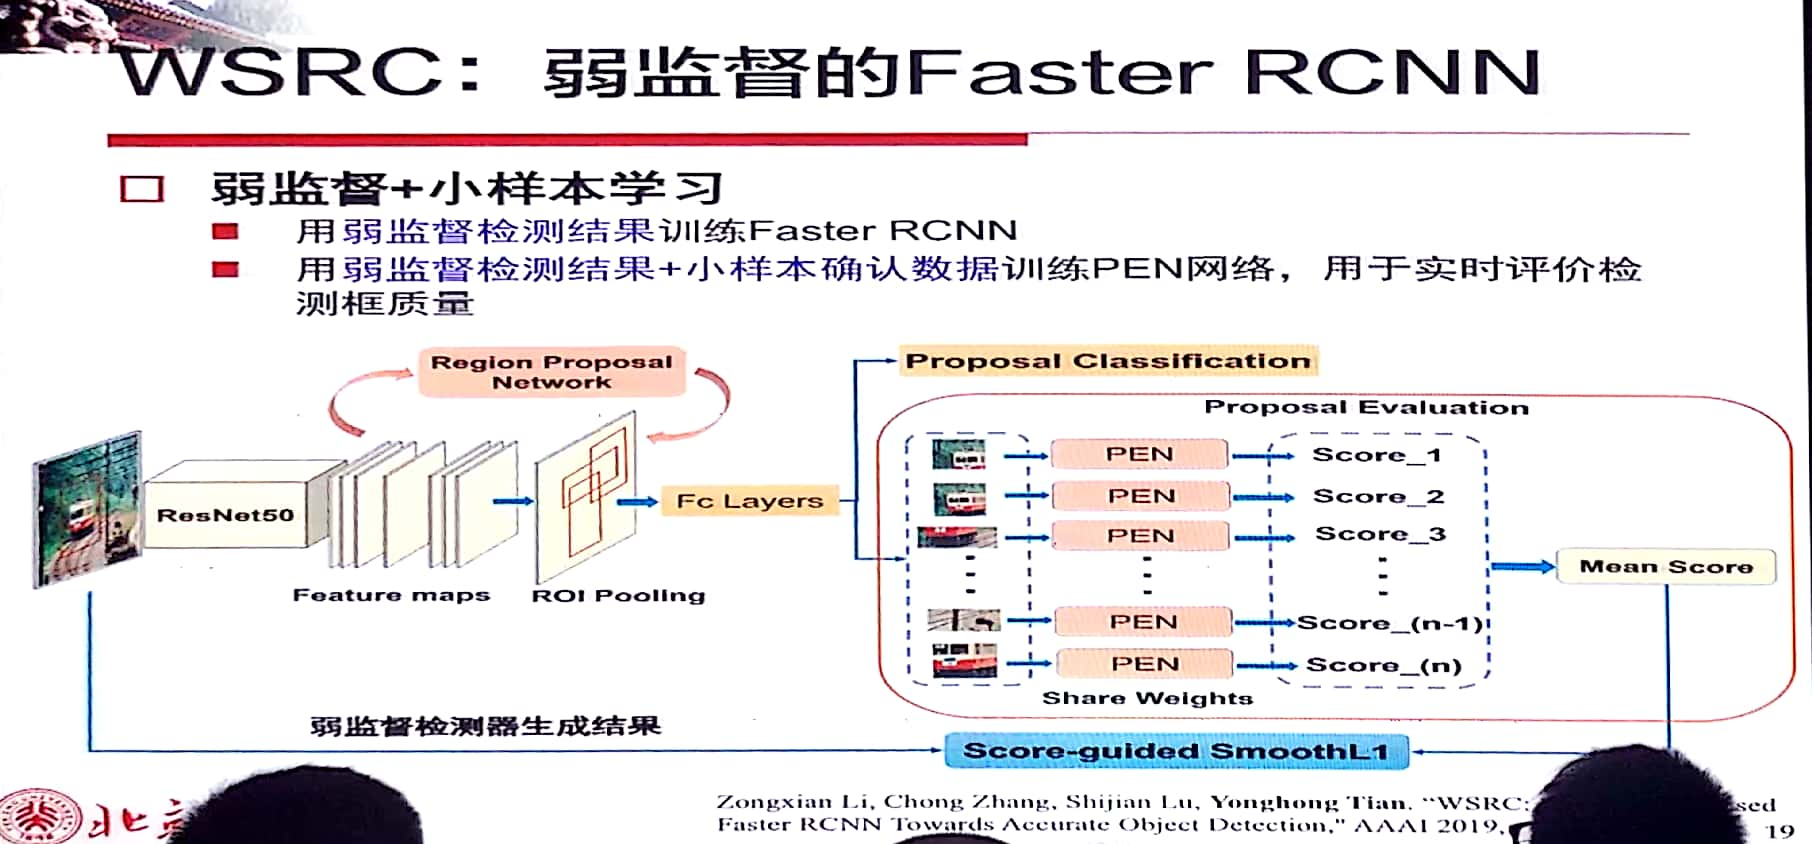
\includegraphics[width=7cm]{figures/1.jpg} 
		} 
		\subfigure[]{ 
			\label{p1b} %% label for second subfigure 
			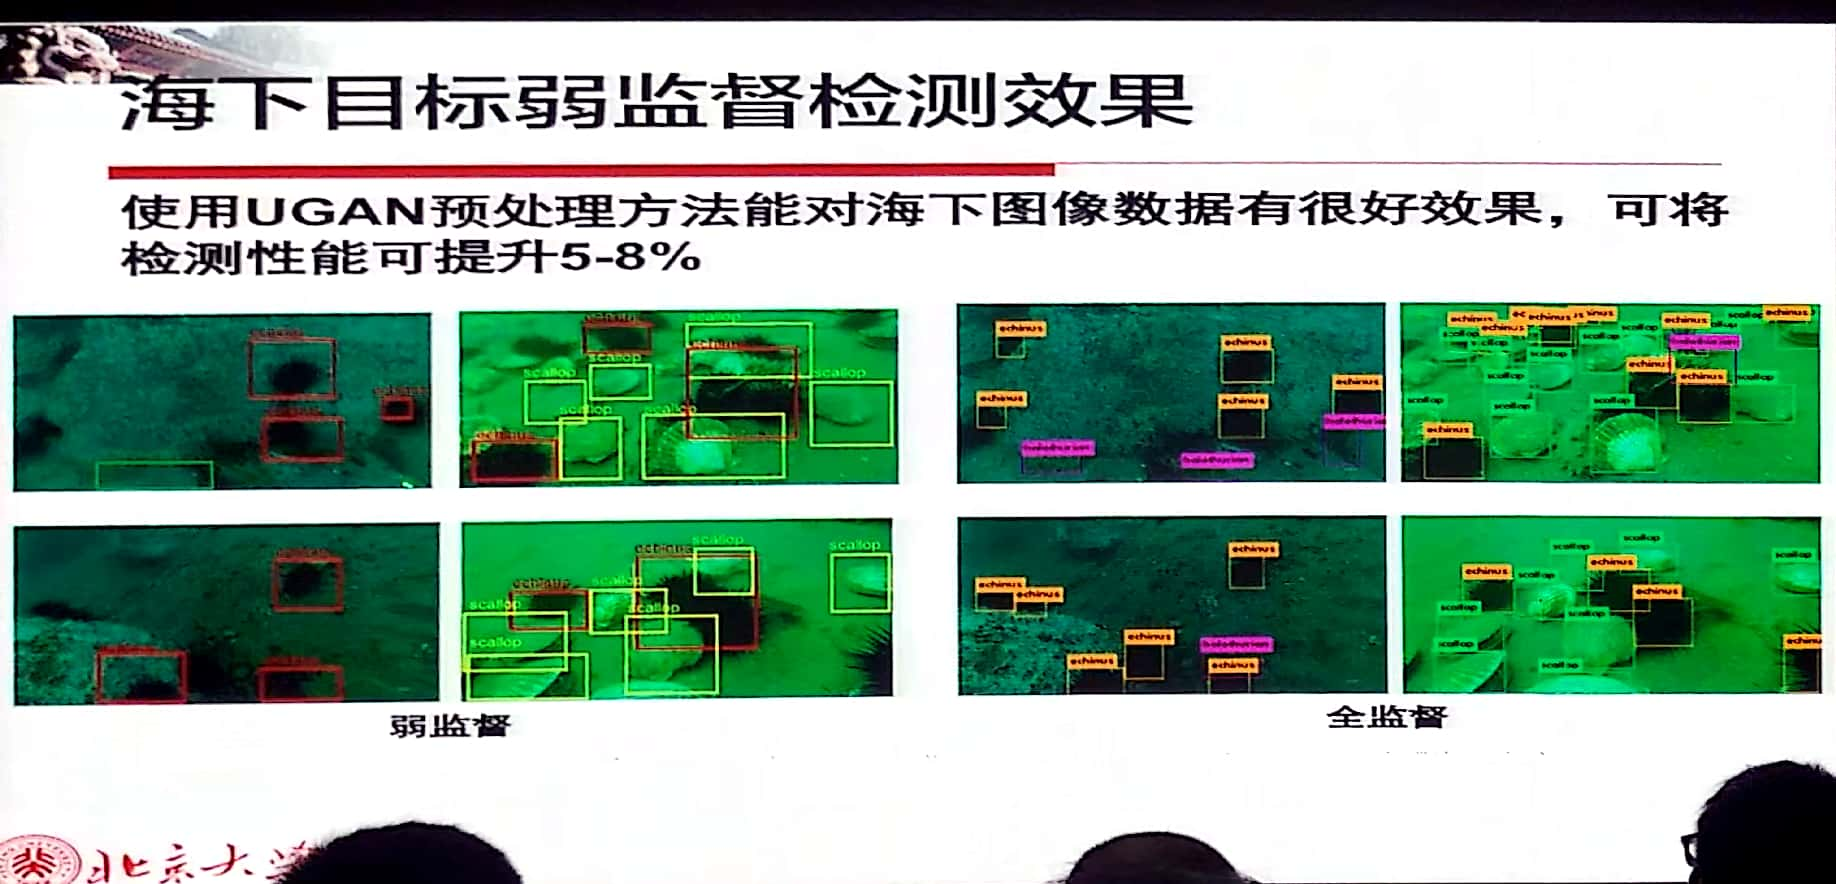
\includegraphics[width=7cm]{figures/2.jpg} 
		}
		\caption{Network architectures and results of WSRC.}
		\label{p1}
	\end{figure}
	
    The undersea target weak supervision detection effectas shown in Fig.~\ref{p1}\subref{p1b}. Finally, we can see this method has a better result than state-of-the-art ones.
    
    Besides, I also learn a new improved algorithm called UGAN as shown in Fig.~\ref{p2}. 
     \begin{figure}
	    \begin{center}
		 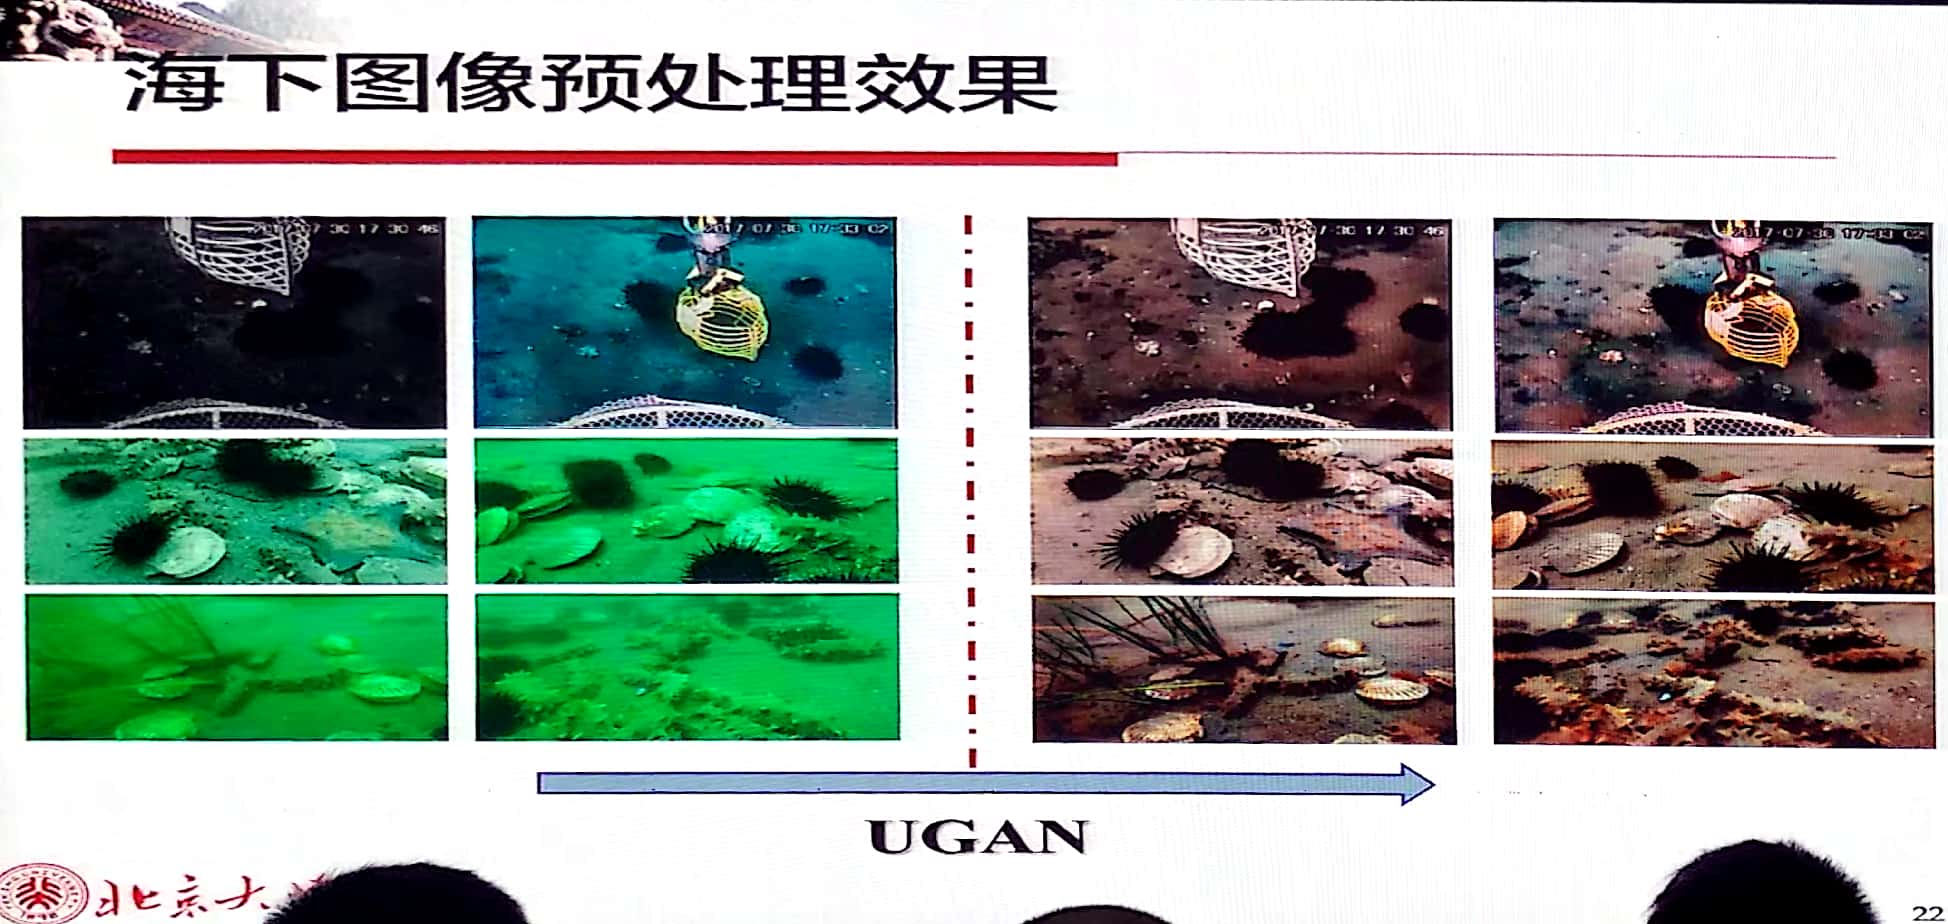
\includegraphics[scale=0.1]{figures/3.jpg}
		\end{center}
		\caption{Underwater image preprocessing effect of UGAN.}
		\label{p2}
	\end{figure} 
	
	\begin{figure}
		\begin{center}
			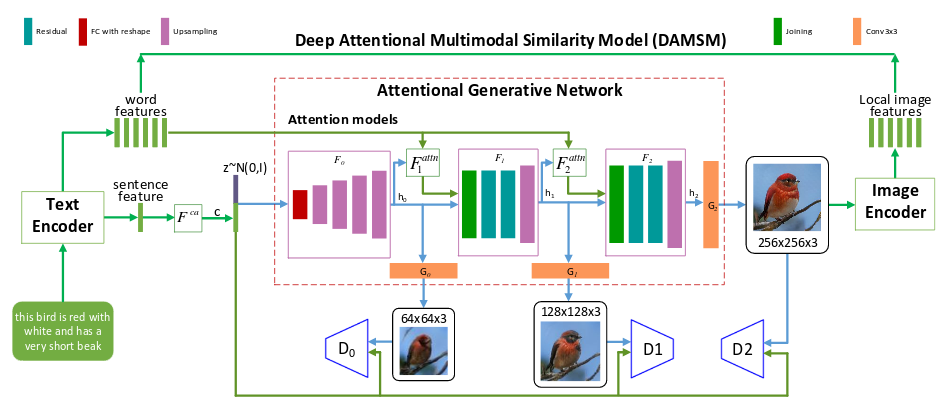
\includegraphics[scale=0.5]{figures/4.png}
		\end{center}
		\caption{The architecture of the proposed AttnGAN. Each attention model automatically retrieves the conditions (i.e., the most relevant	word vectors) for generating different sub-regions of the image; the DAMSM provides the fine-grained image-text matching loss for the generative network}
		\label{p3}
	\end{figure}
	
	\begin{figure}
		\begin{center}
			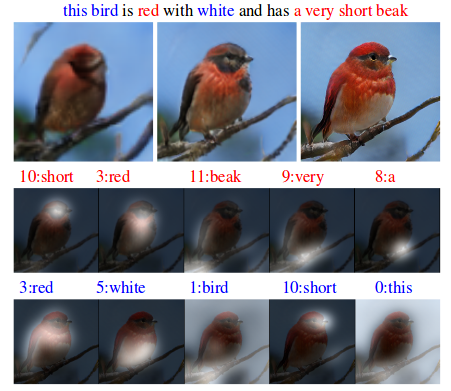
\includegraphics[scale=0.5]{figures/5.png}
		\end{center}
		\caption{Example results of the proposed AttnGAN. The first row	gives the low-to-high resolution images generated by G$_0$, G$_1$ and	G$_2$ of the  AttnGAN; the second and third row shows the top-5 most attended words by F$^{attn}_1$ and F$^{attn}_2$ of the AttnGAN, respectively. Here, images of G$_0$ and G$_1$ are bilinearly upsampled to have the same size as that of G$_2$ for better visualization.}
		\label{p4}
	\end{figure}
	
	\subsection{Text-to-Image Convertor of AttnGAN}
	
	This week, I begin learn about Attentional Generative Adversarial Network (AttnGAN) that allows attention-driven, multi-stage refinement for fine-grained text-to-image generation. With a novel attentional generative network, the AttnGAN can synthesize fine-grained details at different subregions of the image by paying attentions to the relevant words in the natural language description. 
	
	In addition, a deep attentional multimodal similarity model is proposed to	compute a fine-grained image-text matching loss for training the generator. The proposed AttnGAN significantly outperforms the previous state of the art, boosting the best reported inception score by 14.14\% on the CUB dataset and 170.25\% on the more challenging COCO dataset. A detailed analysis is also performed by visualizing the attention layers of the AttnGAN. It for the first time shows that the layered attentional GAN is able to automatically select the condition at the word level for generating different parts of the image.
	
	\lstset{language=python}
	\begin{lstlisting}
	def train(dataloader, cnn_model, rnn_model, batch_size,
	labels, optimizer, epoch, ixtoword, image_dir):
	cnn_model.train()
	rnn_model.train()
	s_total_loss0 = 0
	s_total_loss1 = 0
	w_total_loss0 = 0
	w_total_loss1 = 0
	count = (epoch + 1) * len(dataloader)
	start_time = time.time()
	for step, data in enumerate(dataloader, 0):
	# print('step', step)
	rnn_model.zero_grad()
	cnn_model.zero_grad()
	
	imgs, captions, cap_lens, \
	class_ids, keys = prepare_data(data)
	
	# words_features: batch_size x nef x 17 x 17
	# sent_code: batch_size x nef
	words_features, sent_code = cnn_model(imgs[-1])
	# --> batch_size x nef x 17*17
	nef, att\_sze = words\_features.size(1), words\_features.size(2)
	# words_features = words_features.view(batch_size, nef, -1)
	
	hidden = rnn_model.init_hidden(batch_size)
	# words_emb: batch_size x nef x seq_len
	# sent_emb: batch_size x nef
	words_emb, sent_emb = rnn_model(captions, cap_lens, hidden)
	
	w_loss0, w_loss1, attn_maps = words_loss(words_features, words_emb, labels,
	cap_lens, class_ids, batch_size)
	w_total_loss0 += w_loss0.data
	w_total_loss1 += w_loss1.data
	loss = w_loss0 + w_loss1
	
	s_loss0, s_loss1 = \
	sent_loss(sent_code, sent_emb, labels, class_ids, batch_size)
	loss += s_loss0 + s_loss1
	s_total_loss0 += s_loss0.data
	s_total_loss1 += s_loss1.data
	loss.backward()
	torch.nn.utils.clip_grad_norm(rnn_model.parameters(),
	cfg.TRAIN.RNN_GRAD_CLIP)
	optimizer.step()
	
	if step % UPDATE_INTERVAL == 0:
	count = epoch * len(dataloader) + step
	
	s_cur_loss0 = s_total_loss0[0] / UPDATE_INTERVAL
	s_cur_loss1 = s_total_loss1[0] / UPDATE_INTERVAL
	
	w_cur_loss0 = w_total_loss0[0] / UPDATE_INTERVAL
	w_cur_loss1 = w_total_loss1[0] / UPDATE_INTERVAL
	
	elapsed = time.time() - start_time
	print('| epoch {:3d} | {:5d}/{:5d} batches | ms/batch {:5.2f} | '
	's_loss {:5.2f} {:5.2f} | '
	'w_loss {:5.2f} {:5.2f}'
	.format(epoch, step, len(dataloader),
	elapsed * 1000. / UPDATE_INTERVAL,
	s_cur_loss0, s_cur_loss1,
	w_cur_loss0, w_cur_loss1))
	s_total_loss0 = 0
	s_total_loss1 = 0
	w_total_loss0 = 0
	w_total_loss1 = 0
	start_time = time.time()
	# attention Maps
	img_set, _ = \
	build_super_images(imgs[-1].cpu(), captions,
	ixtoword, attn_maps, att_sze)
	if img_set is not None:
	im = Image.fromarray(img_set)
	fullpath = '%s/attention_maps%d.png' % (image_dir, step)
	im.save(fullpath)
	return count
	\end{lstlisting}\label{g1}
	
	The overall architecture of the AttnGAN is illustrated in Fig.~\ref{p3}.  The model consists of two novel	components. The first component is an attentional generative network, in which an attention mechanism is developed for the generator to draw different sub-regions of the image by focusing on words that are most relevant to the	sub-region being drawn as shoen in Fig.~\ref{p4} and the training code can be seen in Algorithm~\ref{g1}. More specifically, besides encoding the natural  language  description into a global sentence vector, each word in the  sentence is also encoded into a word vector. The generative  network  utilizes the global sentence vector to generate a low-resolution image  in  the first stage. 
	
	In the stages, it uses the image vector in each sub-region to query word vectors by using an attention layer to form a word-context vector. It then combines the regional image vector and the corresponding word-context vector to form a multimodal context vector, based on which the model generates new image features in the surrounding sub-regions. This effectively yields a higher resolution picture with more details at each stage. The other component in the AttnGAN is a Deep Attentional Multimodal Similarity Model (DAMSM). With an attention	mechanism, the DAMSM is able to compute the similarity	between the generated image and the sentence using both	the global sentence level information and the fine-grained word level information. Thus, the DAMSM provides an additional fine-grained image-text matching loss for training the generator. 
	
	
	 
		
	\section{Plan}
	
	\begin{tabular}{rl}
		\textbf{Objective:} & Finish thesis with senior students for CVPR2019.\\
		\textbf{Deadline:} & 2018.11.16
	\end{tabular}
	
	\begin{description}
		\item[\normalfont 2018.09.03---2018.09.09] Finish reading CVPR2018 paper about AttnGAN \cite{Tao18attngan}.
		\item[\normalfont 2018.09.10---2018.09.16] Finish recurrenting results of benchmark table from CVPR2018 paper.
	\end{description}
	
	% If you don't cite any references, please comment the following two lines
	\bibliographystyle{ieee}
	\bibliography{ref.bib}
	
\end{document}